\section*{\Huge{Nomenclature}}
\begin{tabular}{ll}
% A&Area of the wing&$m^{2}$\\
% B\\
% C& Roman letters first, with capitals\ldots\\
% a&then lower case.\\
% b\\
% c\\
% $\Gamma$&Followed by Greek capitals\ldots\\
% $\alpha$&then lower case greek symbols.\\
% $\beta$\\
% $\epsilon$\\
% TLA&Finally, three letter acronyms and other abbreviations arranged alphabetically\\
CNN & Convolutional Neural Network \\
FCN & Fully Convolutional Neural Network \\
LBS & Linear Blend Skinning \\
MSE & Mean Square Error \\
ROI & Region Of Interest \\
&\\
% $\bm{Z}_{m,n}$ & Individual pixel from a depthmap image\\
$\bm{\mathrm{D}}^t$ & Training dataset, where $\bm{\mathrm{D}}^t_k\in\bm{Z}$\\
$\bm{\mathrm{D}}^v$ & Test dataset, where $\bm{\mathrm{D}}^v_k\in\bm{Z}$\\
$E$ & Performance metric \\
$\bm{v}$ & 3D centre of hand in depthmap image $\bm{Z}$, where $\bm{v}\in \mathbb{R}^3$\\
$\bm{\mathrm{Y}}^{i}$ & Groundtruth hand joints, where $\bm{\mathrm{Y}}^{i}_{n} \equiv \bm{\Phi}$, $\bm{\mathrm{Y}}^{i}_{n,m} \equiv \bm{\Phi}_{m}$\\
$\bm{\mathrm{Y}}^{o}$ & Predicted hand joints, where $\bm{\mathrm{Y}}^{o}_{n} \equiv \bm{\Phi}$, $\bm{\mathrm{Y}}^{o}_{n,m} \equiv \bm{\Phi}_{m}$\\
$\bm{Z}$ & Depthmap image, where $\bm{Z}_{m,n} \in \mathbb{N}$ \\

$\bm{\beta}$ & MANO Hand shape parameter, where $\bm{\beta} \in \mathbb{R}^{10}$ \\
$\bm{\theta}$ & MANO hand pose parameter, where $\bm{\theta} \in \mathbb{R}^{45}$\\
$\bm{\Phi}$ & Hand joints, where \bm{$\Phi}=\{\bm{\Phi}_1, \bm{\Phi}_2, ..., \bm{\Phi}_N\}, \bm{\Phi}_{n} \in \mathbb{R}^{3}$\\
&\\
$a$& A scalar value\\
$\bm{a}$ & A vector value\\
$\bm{A}$ & A matrix value\\
$\bm{\mathrm{A}}$ & A tensor value\\
&\\
Articulation & The particular position of the fingers of a hand with respect to each other.\\
Annotation & The marked groundtruth for a depthmap $\bm{Z}$.\\
Groundtruth & True value for $N$ keypoints.\\
Joint & A type of keypoint.\\
Keypoint & Known reference point in a hand in 3D cartesian space.\\
Point Cloud & A series of 3D points which together describe the shape of a 3D surface.\\
Pose & An alternative name for articulation.\\
Prediction & Prediction of the keypoints from a hand tracking model.\\
&\\
\end{tabular}\\
{\bfseries All notation follows the convention set by \cite{goodfellow2016deep}.}

\section*{\Huge{Conventions}}

\begin{figure}[h]
    \renewcommand\thefigure{0.1}
    \centering
    
\includegraphics[width=0.5\linewidth]{figs/general/box_standard.pdf}
    \caption{Box diagram convention. All boxes flow from left to right. Green boxes denote data, and red boxes denote a process on that data.}
\end{figure}

\begin{figure}[h]
    \renewcommand\thefigure{0.2}
    \centering
    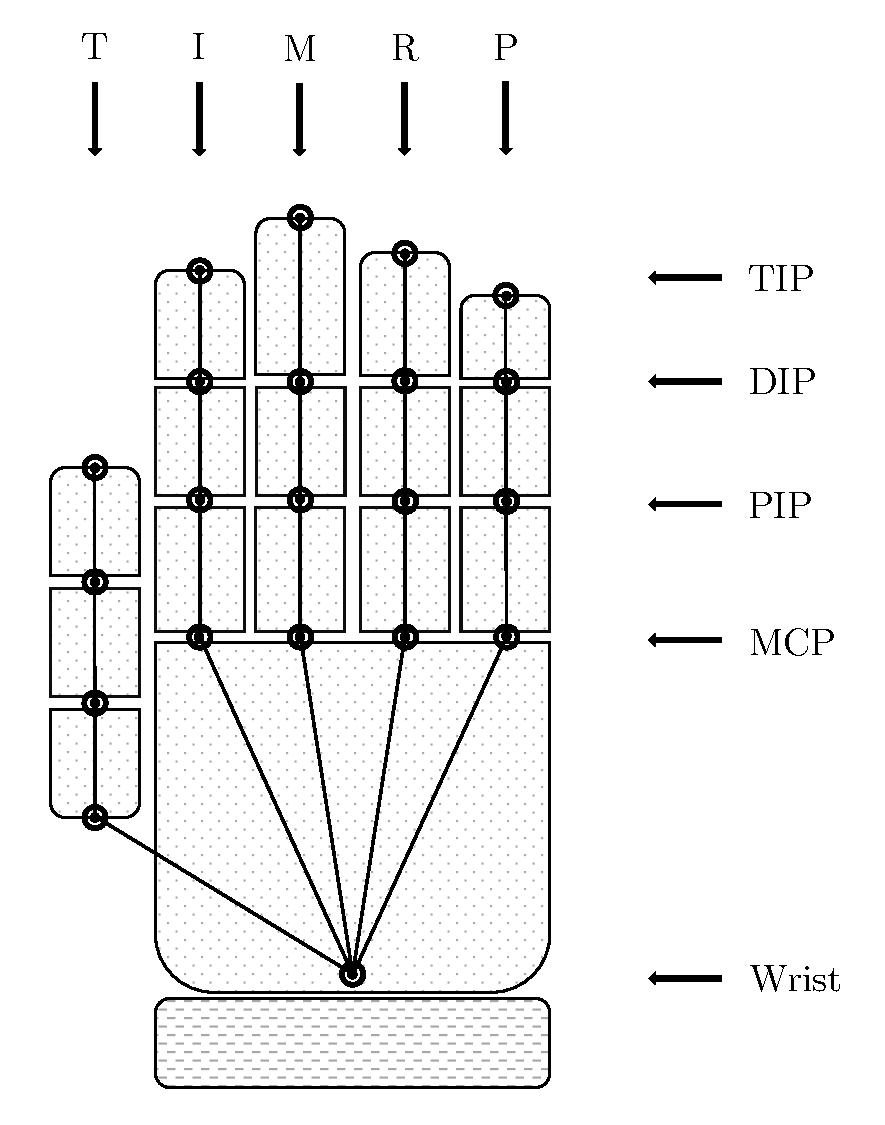
\includegraphics[width=250px]{figs/general/hand_schematic.pdf}
    \caption{Schematic of hand and keypoints. The goal of a hand tracking system is to predict the 3D locations of these keypoints. A keypoint name is the combination of the finger name and joint type, for example, the MCP joint of the Index finger is called the IMCP keypoint. Each of these keypoint names has an equivalent index in $\bm{\Phi}$. From left to right, the finger names used are: thumb, index, middle, ring, and pinky.}
    \label{fig:sd:hand}
    \end{figure}

\vspace{2cm}

% Point cloud?
% Grountruth

% If a parameter has a typical unit that is used throughout your report, then it should be included here on the right hand side.

% If you have a very mathematical report, then you may wish to divide the nomenclature list into functions and variables, and then sub- and super-scripts.

% Note that Roman mathematical symbols are typically in a serif font in italics.